\chapter{Konkurencija i poređenje}

\epigraph{
  Svako je genije. Ali ako ribi sudiš na osnovu toga kako se penje na drvo, živeće ceo život misleći da je glupa.
}{nepoznat autor}

Kao što je već diskutovano u prvom poglavlju, postoji mnogo Javaskript frejmvorka za razviće jednostraničnih veb-aplikacija.
Sem toga, pojam generisanja koda nije nov i masovno se koristi u industriji, prvenstveno kroz bandlere kao što su Vebpek i Rolap.

U ovom odeljku izabrano je nekoliko frejmvorka u kojima je implementirana identična \textquote{Todo} aplikacija kako bi se uporedile neki aspekti performansi postojećih frejmvorka sa Vejnom.

\section{O poređenju}

Pre svega, treba istaći da Vejn u trenutnoj verziji nema ni blizu dovoljno osobina koje ga mogu čini konkurentom postojećih frejmvorka.
U pitanju je prototip koji služi za demonstraciju statičke analize prilikom generisanja koda.

Osim toga, sam pojam poređenja performansi nije jednostavno definisati, a pogotovo ne sa veb-aplikacijama.
Kod prolazi kroz mnoge faze, a postoji i mnogo faktora koji utiču na performanse, od kojih mnogi nisu direktno vezani za frejmvork.

Na primer, dobro podešeno keširanje na serveru i dobro iskorišćen CDN mogu znatno da skrate vreme koje je potrebno da kôd dospe kod klijenta.
Ukoliko server koristi protokol HTTP2, moći će inicira slanje aseta pre nego što ih klijent zatraži.
Brzina izvršenja koda zavisi od snage uređaja na kome se on izvršava i od raspoložive količine RAM memorije.

Pored toga, termin \textquote{performanse} može se odnositi na mnogo toga.
Od trenutka kada korisnik poželi da vidi aplikaciju postoji nekoliko ključnih trenutaka koji mogu biti od koristi prilikom merenja performansi.

Koliko brzo može da \textbf{dođe do nje} je pitanje koje na prvi pogled nije od velike važnosti.
Međutim, poslednjih godina se javlja pojam PWA (\textsl{Progressive Web Application}, progresivna veb-aplikacija) koji korisnicima omogućava da veb-aplikaciju instaliraju na mobilnim uređajima kao da je klasična aplikacija.
Ovo je u neku ruku optimizacija iz ugla korisničkog iskustva i iz ugla većih šansi da se korisik vrati na aplikaciju.

Nakon iniciranja zahteva, treba \textbf{pribaviti određene asete}.
Već ovaj korak prourokuje probleme prilikom definisanja performansi, jer nije jasno određeno \emph{koji} aseti treba da budu dostupni.
Da li je dovoljno da se na ekranu prikaže bilo šta?
Odgovor na ovo pitanje je još teži kada se uzme u obzir da bandleri danas nude mogućnost \textit{deljenja koda} na manje delove, uglavnom po rutama kroz koje se korisnik kreće.
Osim toga, važno je uzeti u obzir tehnike kompresije kao što su \textit{gzip} i \textit{brotli} koje takođe utiču na količinu podataka koju je potrebno prenesti od servera do klijenta.

Nakon što se kod dovuče sa servera, treba ga parsirati i izvršiti.
Međutim, Javaskript nije jedini, a svakako ne primarni, način da se aplikacija renderuje na ekran.
HTML datoteka može već sadržati neki deo interfejsa pre nego što se dovuku Javaskript aseti.
Osim toga, takav HTML može odmah biti interaktivan u potpunosti, delimično interaktivan ili potpuno neinteraktivan.
Da li treba prikazati \textit{ceo} interfejs?
Kao jedna od metrika se često navodi \textbf{prvo crtanje} (\textsl{first paint}) na ekran, ali se takvi rezultati mogu pogrešno protumačiti jer ne govore ništa o interaktivnosti.

Zbog svega ovoga, nije moguće jasno definisati \textquote{pobednika} nad identičnom aplikacijom, što znači da je apsolutno nemoguće govoriti o \textquote{najboljem frejmvorku}, pogotovo kada se uzme u obzir da onda uz performanse pridodaje i iskustvo autora aplikacije (developera) tokom njegovog razvića, što je individualna procena i zavisi od znanja koje je developer ranije stekao, kao i od ličnih preferenci.

Osim toga, frejmvorci mogu biti namenjeni različitim tipovima aplikacija, pa njen izbor može značajno uticati na privid rezultata bilo kakvog poređenja.
Osim tipa, frejmvoci mogu očekivati različite veličine aplikacija i šablona i pristupa koje se od developera očekuje da koristi -- na primer, \textsl{Angular} dolazi uz \textsl{RxJS}, što je biblioteka koja nudi mogućnost rada sa tokovima podataka koristeći šablone funkcionalnog programiranja.

Neki frejmvorci su, na primer, jednostavniji za testiranje od drugih.
Štaviše, neki mogu biti jednostavniji za pisanje junit testova (\textsl{Hyperapp}), a neki za pisanje integracionih ili sistemskih testova (\textsl{Angular}).
Neki \textquote{frejmvorci} uopšte nisu frejmvorci već biblioteke za koje se očekuje da se koriste uz razne druge biblioteke kako bi se dobio utisak rada sa frejmvorkom (\textsl{React} se obično koristi uz \textsl{Redux}, \textsl{React Router} i neku biblioteku za pisanje CSS-in-JS stilova ili pak vebpek transformer za učitavanje stilova iz \code{.css} datoteke).

Postoje frejmvorci koji mogu da se koriste dirketno pomoću \code{script} taga bez gubitka performansi i postoje frejmvorci koji su projektovani tako da se oslanjaju na alate koji će moći da obave neophodne transformacije koda u cilju minifikacije.

Ovo su samo neke od osobina koje mogu uticati na izbor frejmvorka.
Cilj ovog poglavlja \textbf{nije da izabere \textquote{najbolji} frejmvork} već da se prilikom poređenja oslikaju sličnosti i razlike sa drugim frejmvorcima, njihovi nedostaci u odnosu na Vejn i njihove prednosti.

Osim toga, nije ulagano vreme u detaljnu analizu izlaznih aseta radi sofisticirane optimizacije promenom načina generisanja izlaznih fajlova.
Za frejmvorke koji dolaze uz CLI koriste se podrazumevana podešavanja, a za one koji ga nemaju iskorišćen je neki od popularnijih startera koji su \textquote{overeni} od strane zajednice.

Imajući ovo u vidu, ostatak poglavlja se bavi isključivo \textbf{veličinom koda} kao metrikom, uz posvrt na -- što je objektivnije moguće -- iskustva developera prilikom razvića aplikacije.

\section{Aplikacija}
\label{subsec:app}

\textquote{Todo} je klasičan primer aplikacije na kome se demonstriraju neke osnovne osobine frejmvorka.
Korisnik na aplikaciji može zabeležiti stavke u listi zadataka koje treba da obavi, svaki od njih može obeležiti kao završen ili opovrgnuti tu naredbu.
Pored toga, moguće je filtrirati listu na osnovu toga da li su zadaci obavljeni ili ne.

Dok nijedna stavka nije dodata u listu, prikazuje se odgovarajuća poruka.
Kada stavki ima, ali nisu vidljive zbog izabranih filtera, takođe se prikazuje poruka u kojoj se pominje ukupan broj postojećih stavki.

Izgled aplikacije prikazan je na slici~\ref{fig:izgled-app}. Kako bi se pažnja usmerila na ključne delove frejmvorka, stilovi su namerno izostavljeni i svedeni na minimum, samo onoliko koliko je potrebno da aplikacija ima smisla.

\begin{figure}
  \centering
  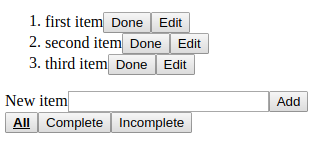
\includegraphics[scale=0.5]{ch06/app.png}
  \caption{Izgled aplikacije za poređenje.}
  \label{fig:izgled-app}
\end{figure}

\subsection{Angular}

\textsl{Angular} je jedan od tri vodeća frejmvorka koji se najčešće koriste u industriji.
Nameće Tajpskript kao jedini zvanični način pisanja aplikacija.
U pitanju je Guglov proizvod.

Osnovna jedinica za izgradnju interfejsa je komponenta, koja se registruje u module iz kojih se može izvesti da bi se koristila u drugim modulima.
Za biznis-logiku i komunikaciju između komponenti koje nisu u predefinisanom roditelj-dete odnosu iz šablona koriste se servisi, koji se koriste u komponentama upotrebom šablona ubrzigavanja zavisnosti (\textsl{dependency injection}.

Komponenta je predstavljena klasom i dekoratorom \code{@Component} u kome se navode meta-podaci o klasi koje \textsl{Angular} koristi da bi \textquote{razumeo} kako komponenta treba da se ponaša u šablonima.

Koristi posebnu šablonsku sintaksu nalik na HTML za definisanje šablona, što ih čini jednostavnim za razumevanje.
Dolazi uz svoj kompajler, \code{ngc}, koji je omotač oko \code{tsc} i služi za generisanje koda za šablone.
Ne bavi se detaljnom analizom koda, već se proces kompilacije koristi kako se parser i kompilator šablona ne bi slao klijentu.

Šablonskom sintaksom se definiše kako javni interfejs komponent komunicira sa tekućom komponentom, a unutar same klase se koriste dekoratori \code{@Input} i \code{@Output} da bi se taj interfejs definisao.

Ima svoj zvaničan CLI koji enkapsulira neophodna podešavanja za okruženje prilikom razvića kao i za produkcioni bild.
Za ovo interno koristi Vebpek, ali je ideja njegove ekapsulacije to da može da se zameni bez uticaja na autore koda.
Postoje planovi da se umesto njega koristi \textsl{Bazel} uz \textsl{Closure Compiler}.

Iniciranje novog projekta svodi se na jednostavno pokretanje komande, a zahvaljujući \textsl{Schematics} sistemu, nude se i komande kojima se mogu generisati potrebne datoteke za kreiranje komponenti.

Korišćenjem šablona ubrizgavanja zavisnosti dobija se kod gde se lako mogu mokovati zavisnosti u testovima.
Postavka testova je već podešena zahvaljujući CLI-ju i uz svaku komponentu generiše se i po jedan podrazumevani junit-test.
Mogu se pisati i sistemski testovi.

Stilovi su automatski enkapsulirani, tj. ograničeni na komponentu.
CLI dolazi uz podršku za \textsl{Sass} koja se može uključiti promenom podešavanja u konfiguracionom fajlu.
Postoji mogućnost deljenja koda na delove na osnovu ruta kako se čitava apilkacija ne bi dovlačila odmah, već po zahtevu korisnika.

Veličina izlaznih Javaskript fajlova je $244741\,\mathrm{b}$ bez kompresije, odnosno $71600\,\mathrm{b}$ i $62670\,\mathrm{b}$ kada se koriste kompresije \textsl{gzip} i \textsl{brotli}, redom.\footnote{\url{https://github.com/lazarljubenovic/todo-app-comparison-angular}} Kompresija daje $3.9$ puta manji kod.

\subsection{React}

\textsl{React} je najpopularnija i u industiji najtraženija biblioteka za razviće korisničkih interfejsa.
Iza nje stoji Fejsbuk.

Interfejs se gradi od komponenti koji se predstavljaju klasom koja nasleđuje klasu \code{React.Component} i implementira metodu \code{render} koja vraća virtuelni čvor.
Za jednostavne komponente može se koristiti i obična funkcija koja direktno vraća virtuelni čvor.

Virtuelni čvorovi mogu se graditi korišćenjem funkcije \code{createElement} (koja se često preimenuje na \code{h} radi kraćeg pisanja).
Međutim, češće se koristi specijalna sintaksa za pisanje šablona koja se naziva JSX.
Ova sintaksa omogućava da se poziv funkcije definiše nalik na definisanje taga u XML-u, što šablonu daje izgled koji podseća na HTML umesto na pozive funkcija.
Ipak, mnogo detalja se razlikuje u odnosu na HTML što zna da dovede do zabune.
Takođe, pošto je u pitanju proizvoljan Javaskript, jednostavno je da se u šablone umeša proizvoljna logika.
S druge strane, postoji velika sloboda koju developer može iskorititi u svoju korist kao prednost.

Mada se radi o biblioteci za pisanje korisničkih interfejsa, ne postoji nijedan zvaničan način kojim se olakšava pisanje CSS-a.
Zajednica je podeljenih mišljenja o tome kako stilove treba pisati -- od tradicionalnog načina sa globalnim stilovima do specijalnih biblioteka koje uopšte ne koriste CSS, već samo Javaskript, tako što stilove definišu \textit{inline}, odnosno direktno nad HTML elementima.

Komponenta se parametrizuje svojstvima koji se prenose kao objekat.
Ne postoji posebna sintaksa za definisanje događaja (\textquote{izlazi} u Vejnu), već se funkcija jednostavno prosleđuje kao svojstvo (slično \textquote{ulazima} u Vejnu).

Kako se radi o biblioteci a ne frejmvorku, sve odluke o organizaciji koda i strukture datoteka prepuštene su developeru.
Sem toga, \textsl{React} sam po sebi nije dovoljno rešenje za pisanje velikih aplikacija, pa se oslanja na eksterne biblioteke koje ga dopunjuju; na primer: za upravljanje stanjem koriste \textsl{Redux} i \textsl{MobX}, za stilove mogu se koristi \textsl{CSS modules}, \textsl{styled-components}, \textsl{emotion}, \textsl{classnames}.
Ne postoji ni zvaničan ruter, već se koristi rešenje zajednice \textsl{React Router}, mada i tu postoje alternative.

Postoji zvaničan CLI pod imenom \textsl{Create React App} kojim se projekat postavlja, ali nema naredbe za generisanje koda za dodatne komponente.

\textquote{Todo} aplikacija implementirana je bez pomoćnih biblioteka jer je dovoljno jednostavna da za time ne postoji potreba.
Veličina izlaznih Javaskript fajlova je $122323\,\mathrm{b}$ bez kompresije, odnosno $38465\,\mathrm{b}$ i $33709\,\mathrm{b}$ kada se koriste kompresije \textsl{gzip} i \textsl{brotli}, redom.\footnote{\url{https://github.com/lazarljubenovic/todo-app-comparison-react}} Kompresija daje $3.6$ puta manji kod.

\subsection{Vue}

\textsl{Vue} je nešto mlađi alat od prethodna dva i, za razliku od njih, ne dolazi iz veće kompanije.
Stekao je veliku popularnost zbog svoje jednostavnosti i skalabilnosti.

U pitanju je hibrid biblioteke i frejmvorka; može se ponašati kao i jedno i drugi u zavinosti od toga kako se koristi.
Jednostavno je dodati ga u postojeći projekat i time deo tradicionalnog veb-sajta učiniti da bude \textsl{Vue} aplikacija, a može se koristiti i za pravljenje jednostraničnih aplikacija.

Aplikaciju čine komponente od kojih se stablo komponenti gradi šalonima koji su nadskup HTML sintakse, slično Angularu.
Za razliku od Angulara, ne postoje moduli za grupisanje komponenti, već se registracija za korišćenje u šablonima vrši na nivou komponente.
S druge strane, moguće je pisati i \code{render} funkciju gde se takođe može koristiti JSX radi jednostavnijeg pisanja, ali se to ne nameće.

Ulazi u komponentu se eksplicitno navode u okviru definicije komponente, što je zapravo objekat sa određenim svojstvima.
Izlazi se ne kreiraju, već se događaji ispaljuju korišćenjem metode \code{\$emit} kojoj se kao prvi argument prosleđuje ime događaja.

Stilovi se mogu enkapsulirati, tj. ograničiti na komponentu.

Komponente se pišu u posebnim SFC datotekama (\textsl{Single File Component}, komponenta u jednoj datoteci), gde su šablon, kod i stilovi u jednoj datoteci, omeđeni XML tagovima \code{template}, \code{script} i \code{style}.

Za implementaciju \textquote{Todo} aplikacije \textsl{Vue} je korišćen kao frejmvork.
Veličina izlaznih Javaskript fajlova je $93980\,\mathrm{b}$ bez kompresije, odnosno $33793\,\mathrm{b}$ i $30177\,\mathrm{b}$ kada se koriste kompresije \textsl{gzip} i \textsl{brotli}, redom.\footnote{\url{https://github.com/lazarljubenovic/todo-app-comparison-vue}} Kompresija daje $3.1$ puta manji kod.

\subsection{Preact}

\textsl{Preact} je \textquote{brza alternativa za \textsl{React} od $3\,\mathrm{kb}$ sa istim modernim API-jem}.
U pitanju je biblioteka koja je nastala sa idejom da iz \textsl{React}-a odbaci neke delove kako bi ostala samo srž, svedena na minimum.
Zbog ovoga deli sve tehničke osobine sa \textsl{React}-om.

Na zvaničnom sajtu nalaze se detaljna upustva za migraciju \textsl{React} koda, što se uglavnom svodi na zamenu imena i nekih jednostavnih transformacija kako bi se zaobišli neki delovi API-ja koje \textsl{Preact} ne podržava.
Opciono se može koristiti modul \code{preact-compat} kojim se jaz između njihovih interfejs\=a dodatno smanjuje, a iznosi $2\,\mathrm{kb}$.

Zajednica je razvila CLI za \textsl{Preact} nazvan analogno onom koji ima \textsl{React}: \textsl{Create Preact App}, koji ima iste osobine kao original.

Zbog jednostavnosti \textquote{Todo} aplikacije, u implementaciji nije bilo problema sa migracijom.
Prevedeni su samo uvozi iz modula tako što je \textsl{react} zamenjeno sa \textsl{preact} i aplikacija je uspešno pokrenuta.
Veličina izlaznih Javaskript fajlova je $29408\,\mathrm{b}$ bez kompresije, odnosno $10756\,\mathrm{b}$ i $9675\,\mathrm{b}$ kada se koriste kompresije \textsl{gzip} i \textsl{brotli}, redom.\footnote{\url{https://github.com/lazarljubenovic/todo-app-comparison-preact}} Kompresija daje $3$ puta manji kod.

\subsection{Hyperapp}

\textsl{Hyperapp} je mikro-frejmvork za razviće jednostraničnih aplikacija.
Veličina koda frejmvorka iznosi svega $1.5\,\mathrm{kb}$.

Kao i \textsl{React}, koristi virtuelni DOM kompatibilan sa JSX sintaksom, ali su ovde komponente isključivo funkcije (ne i klase).
Koncept stanja komponenti ne postoji, već se stanje čuva u skladištu koje je globalno za celu aplikaciju, odakle komponente mogu uzimati delove stanje koje su neophodne za renderovanje korisničkog interfejsa.
Takođe, komponente mogu ispaliti akcije kojima se skladište ažurira na \textit{immutable} način.
Suštinski se radi o kombinaciji \textit{React}-a i \textit{Redux}-a u jednom.

Zbog svoje jednostavnosti, ne postoji zvaničan CLI.
Dokumentacija frejmvorka je dovoljna da se brzo izvrši optimalna postavka.
Veličina izlaznih Javaskript fajlova je $6378\,\mathrm{b}$ bez kompresije, odnosno $2599\,\mathrm{b}$ i $2336\,\mathrm{b}$ kada se koriste kompresije \textsl{gzip} i \textsl{brotli}, redom.\footnote{\url{https://github.com/lazarljubenovic/todo-app-comparison-hyperapp}} Kompresija daje $2.7$ puta manji kod.

\subsection{Wane}

\textsl{Wane} je opisan u ranijim poglavljima.

Veličina izlaznih Javaskript fajlova je $16904\,\mathrm{b}$ bez kompresije, odnosno $3475\,\mathrm{b}$ i $3064\,\mathrm{b}$ kada se koriste kompresije \textsl{gzip} i \textsl{brotli}, redom.\footnote{\url{https://github.com/lazarljubenovic/todo-app-comparison-wane}} Kompresija daje $5.5$ puta manji kod.

\section{Analiza rezultata}
\label{sec:analiza}

Rezultati su, jednom rečju, \emph{očekivani}.
Tabelarno i grafički su prikazani u tabeli~\ref{tab:analiza} i na slici~\ref{fig:analiza}.

\textsl{Angular}, kao najglomazniji frejmvork koji nudi sve što je neophodno za razviće ozbiljne jednostranične aplikacije.
Nije zamišljen da se koristi za izgradnju jednostavnih aplikacija kao što je ova, što se ogleda i u veličini koda.

Prate ga \textsl{React} i \textsl{Vue}, pri čemu je veličina React koda nešto veća, što možda dovodi u njegovu pitanje \textquote{minimalnost}, s obzirom da se radi o biblioteci a ne o frejmvorku.

\textsl{Preact} pokazuje značajno smanjenje koda u odnosu na React bez ikakve promene, što opravdava način na koji se reklamira.

\textsl{Hyperapp} pokazuje najmanju veličinu koda.
Takođe, on je jedini primer frejmvorka u kome je autorov kod dominantan nad kodom frejmvorka, što znači da je jedino u ovom slučaju načinjen pravi izbor po pitanju izbora frejmvorka za ovako jednostavnu aplikaciju.

\textsl{Wane} pokazuje izuzetno mali kod, ali ne manji od onog koji se dobija iz \textsl{Hyperapp} koda, što znači da i pored svog potencijala, \textsl{Wane} trenutno nije spobodan da dovoljno optimizuje kod, što bi posebno došlo do izražaja u većoj aplikaciji kod kojih rast veličine koda \textsl{Hyperapp} aplikacije može da bude samo linearano srazmeran veličini autorovog koda, dok se kod \textsl{Wane} aplikacije očekuje strmiji rast (mada ovo nije lako predvideti u praksi zbog korišćenja kompresije koja je mnogo izraženija u \textsl{Wane} aplikacije -- postoji mogućnost da će rast \textsl{Wane} bandla sa porastom aplikacije biti logaritamski i da će u nekom ternutku nadmašiti \textsl{Hyperapp} koji ima manjih šansi za grublju kompresiju).

Zanimljivo je zapaziti kako je izlazni kod svih frejmvorka kompresija dala oko tri puta manji kod, osim u slučaju kada je za pisanje aplikacije korišćen \textsl{Wane}, kod koga je odnos kompresije veći od pet.
Ovo je posledica toga što je u \textsl{Wane} aplikaciji kod generisan, što znači da često ima ponavljanja.
Osim toga, za jednostavne slučajeve \textsl{Wane} kompilator generiše odmotane petlje; na primer, prilikom generisanja enkapsulacije za stilove, ne pušta se petlja već se ispiše nekoliko izraza koji se razlikuju samo po indeksu.
Ovo daje veći kôd nego da je korišćena generalna funkcija ili \code{for} petlja, ali zato daje bolju kompresiju i u teroiji bolje performanse jer se pozivi funkcjia retko mogu nagomilati (mada je ova prednost u praksi najčešće potpuno zanemarljiva).

\begin{table}[p]
  \centering
  \begin{tabularx}{0.66\textwidth}{Xrrr}
    \toprule 
    \textsc{Frejmvork} & {raw} & {gzip} & {brotli} \\
    \midrule
    \textbf{Angular} & $244~741$ & $71~600$ & $62~670$ \\
    \textbf{React}   & $122~323$ & $38~465$ & $33~709$ \\
    \textbf{Vue}     &  $93~980$ & $33~793$ & $30~177$ \\
    \textbf{Preact}  &  $29~408$ & $10~756$ &  $9~675$ \\ 
    \textbf{Hyperapp}&   $6~378$ &  $2~599$ &  $2~336$ \\
    \textbf{Wane}    &  $16~904$ &  $3~475$ &  $3~064$ \\
    \bottomrule
  \end{tabularx}
  \caption{Rezultati analize veličine koda aplikacije \textquote{Todo} implementirane u šest frejmvorka. Sve brojne vrednosti su u bajtovima. Grafički prikaz rezultata prikazan je na slici~\ref{fig:analiza}, a diskusija istih nalazi se u~\cref{sec:analiza}.}
  \label{tab:analiza}
\end{table}

\begin{figure}[p]
  \centering
  \begin{bchart}[step=10,max=80]
    \bcbar[color=black!10, text=gzip]{71.6}
    \bclabel{Angular}
    \bcbar[color=black!10, text=brotli]{62.6}
    \smallskip
    \bcbar[color=black!10, text=gzip]{38.4}
    \bclabel{React}
    \bcbar[color=black!10, text=brotli]{33.7}
    \smallskip
    \bcbar[color=black!10, text=gzip]{33.8}
    \bclabel{Vue}
    \bcbar[color=black!10, text=brotli]{30.1}
    \smallskip
    \bcbar[color=black!10, text=gzip]{10.8}
    \bclabel{Preact}
    \bcbar[color=black!10, text=brotli]{9.7}
    \smallskip
    \bcbar[color=black!10, value={2.6 (gzip)}]{2.6}
    \bclabel{Hyperapp}
    \bcbar[color=black!10, value={2.3 (brotli)}]{2.3}
    \smallskip
    \bcbar[color=black!10, value={3.5 (gzip)}]{3.5}
    \bclabel{Wane}
    \bcbar[color=black!10, value={3.0 (brotli)}]{3.0}
  \end{bchart}
  \caption{Rezultati analize veličine kompresovanog koda aplikacije \textquote{Todo} implementirane u šest frejmvorka u hiljadama bajtova. Gornji stubac predstavlja \textsl{gzip}, a donji \textsl{brotli} kompresiju. Tabelarni prikaz rezultata prikazan je u tabeli~\ref{tab:analiza} zajedno sa veličinom datoteka pre kompresije, a diskusija istih nalazi se u~\cref{sec:analiza}.}
  \label{fig:analiza}
\end{figure}
